\chapter{实现}

本章主要介绍\todo{。。}

\section{整体架构}

章\ref{sec:fl_frame}中已经描述了本文要实现的缺陷定位框架。
这个缺陷定位框架如图\ref{fl_frame1}所示,一共包含三个大的模块:
谓词生成模块,频谱信息收集模块,和怀疑度计算模块。
\begin{figure}[htbp] 
\centering 
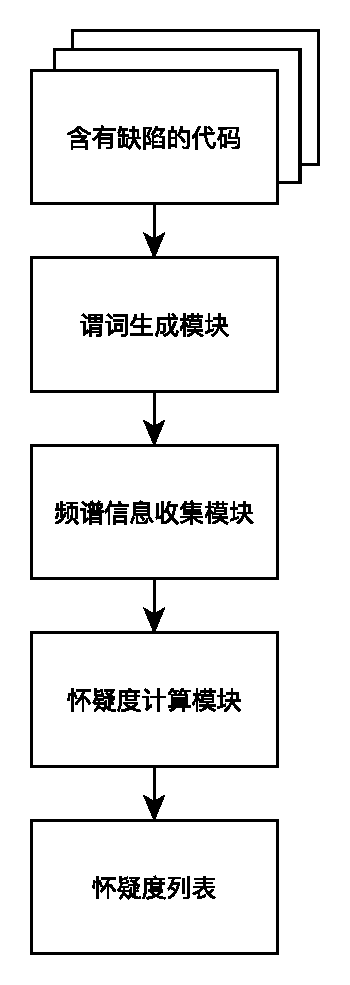
\includegraphics[width=5cm]{figure/frame1} 
\caption{缺陷定位框架模块图} 
\label{fl_frame1}
\end{figure}

谓词生成模块生成预定义的谓词,或者利用机器学习模型预测出谓词。
频谱信息收集模块把生成的谓词插装到缺陷代码,执行测试用例,收集测试用例覆盖谓词真假分支的情况。
最后怀疑度计算模块利用频谱信息,带入公式中计算怀疑度。

具体的流程图如图\ref{fl_frame2}所示。下面将会具体讲述这些步骤的实现。

\begin{figure}[htbp] 
\centering 
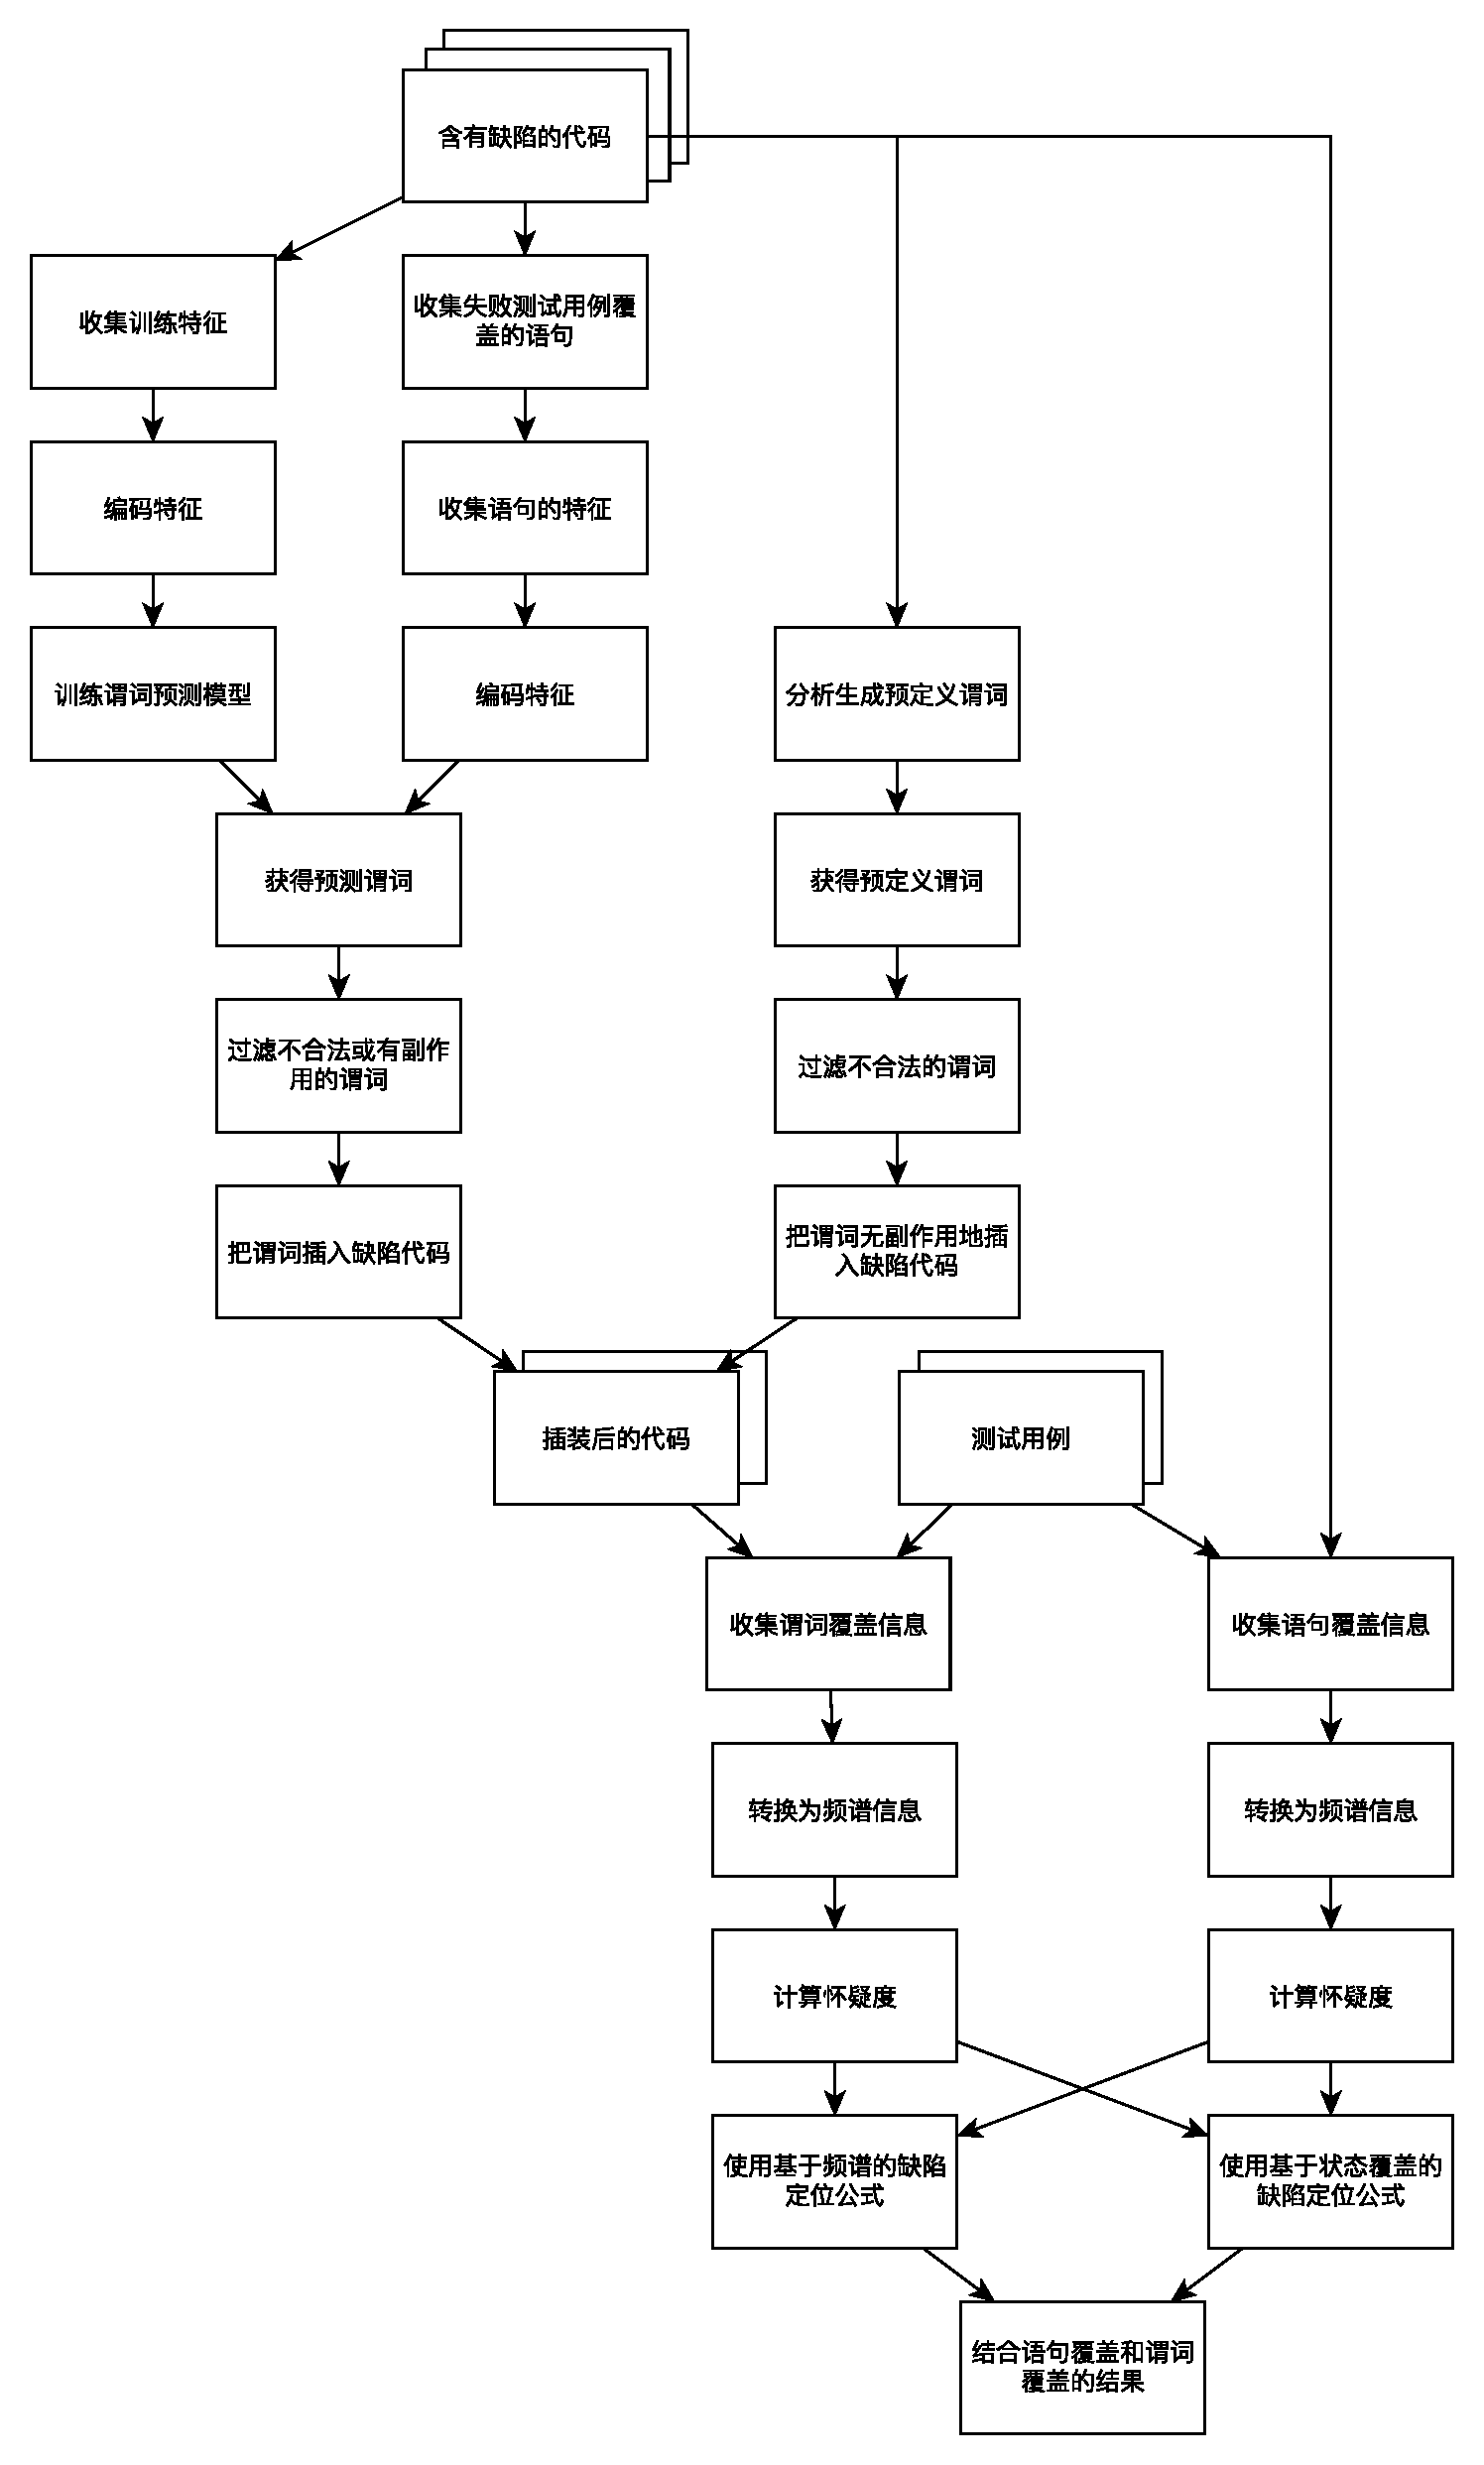
\includegraphics[width=13cm]{figure/frame2} 
\caption{缺陷定位整体流程图}
\label{fl_frame2}
\end{figure}

\section{谓词生成模块}

谓词生成模块负责生成后续会使用的谓词.
谓词生成模块分为两种,一种是生成预测谓词,一种是生成预定义谓词。
生成谓词的语句都是被失败的测试用例覆盖的语句。

\subsection{生成预测谓词模块}

生成预测谓词使用的是机器学习模型,使用Java和Python实现。
首先,Java代码通过JDT遍历缺陷代码的抽象语法树,提取表\ref{var_feature}中的特征。
这些特征被写入到磁盘上的 csv 文件中。
Python程序则读入 csv 文件中的特征,对特征进行编码和训练。

编码阶段,先对变量名、文件名、函数名使用scikit-learn\footnote{\url{http://scikit-learn.org/}}的K-Means聚类,其值转为类编号。
聚类模型等被存储到磁盘。
使用 scikit-learn 的 \mycode{LabelEncoder} 对特征 FileName,MethodName,VarName,VarType,LastAssign,BodyUse
和 OutUse 进行编码,归一化为数字,然后使用 \mycode{OneHotEncoder} 转为独热编码。

训练阶段,特征被放入神经网络或者决策树中。
神经网络使用的全连接神经网络,用TensorFlow\footnote{\url{https://www.tensorflow.org/}}的 \mycode{DNNClassifier} 实现。
TensorFlow 是一个采用数据流图用于数值计算的开源软件库。
图中的节点表示数学操作,图中的线则表示在节点间相互联系的多维数据数组。
网络的输入使用 TensorFlow 的 \mycode{numpy\_input\_fn}。
使用这个函数的好处是,输入不需要在一开始的时候就被存储在内存,
而是在需要的时候才生成一个批(batch)的数据。
每次训练以一个批的数据为一次迭代。
VAR模型和EXPR模型的批尺寸(batch size)都为128。
输入数据会被随机打乱(shuffle)。
一个周期(epoch)就是把全部数据输入神经网络训练一次。
输入数据按照$7:3$的比例分为训练集和验证集。
训练时,会先使用训练集训练\mycode{INIT\_EPOCHS}个周期。
这是因为训练开始时,损失变化较大。
此后每次都再输入一个周期,并收集训练集和验证集在输入这个周期后的新模型上的损失和准确率。
程序会收集最近的\mycode{1}到\mycode{2 * TEST\_EPOCHS}个周期的
训练集和验证集的损失,记为$L(i, j)$。
其中$i$表示是最近的第$i$个周期的损失,$j$为$true$的话表示是训练集的损失,为$false$表示是验证集的损失。
然后分别计算\mycode{1}到\mycode{TEST\_EPOCHS},\mycode{TEST\_EPOCHS + 1}到\mycode{2 * TEST\_EPOCHS}
的训练集总损失值
$$
Loss_1 = \mathrm{Loss}(1, TEST\_EPOCHS, true)
$$
$$
Loss_2 = \mathrm{Loss}(TEST\_EPOCHS + 1, 2 * TEST\_EPOCHS, true)
$$
和验证集的总损失值
$$
Loss_3 = \mathrm{Loss}(1, TEST\_EPOCHS, false)
$$
$$
Loss_4 = \mathrm{Loss}(TEST\_EPOCHS + 1, 2 * TEST\_EPOCHS, false)
$$。
其中$\mathrm{Loss}$定义如下:
$$
\mathrm{Loss}(start, end, j) = \sum_{i=start}^{end}{L(i, j)}
$$。
终止训练的条件为
$$
Loss_1 < Loss_2 \ \mathrm{and} \ Loss_3 > Loss_4
$$。
也就是说当训练集的损失仍在下降,但是验证集的损失却开始上升时,
说明出现了过拟合,停止训练。
训练时会记录当前最小的验证集损失,并会把对应的模型存入磁盘。
训练停止后,最小损失对应的模型成为最终模型。
训练使用 \mycode{DNNClassifier} 的 \mycode{train} 方法,
验证损失和准确率使用 \mycode{evaluate} 方法。
神经网络使用的优化算法是 \mycode{ProximalAdagradOptimizer},
初始学习率设置为0.05,l2正则系数为0.0001。、
决策树使用 scikit-learn 中的决策树 \mycode{DecisionTreeClassfier} 。
训练使用其 \mycode{fit} 方法。
训练好的模型被保存在磁盘中。
神经网络模型直接通过设置 \mycode{model\_dir} 参数保存,
决策树模型使用 pickle\footnote{\url{https://docs.python.org/3/library/pickle.html}} 保存。

预测阶段,对收集的失败测试用例覆盖的语句进行谓词预测。
首先用Java的JDT提取语句中左值变量的特征,然后写入磁盘上的 csv 文件。
Python程序读入 csv 文件中的特征和编码阶段存储的聚类模型。
同时Python程序也会读入训练时使用的 csv 文件,以获取同样的 \mycode{LabelEncoder} 和 \mycode{OneHotEncoder}。
使用聚类模型对特征的变量名、函数名和文件名划入某个已有的分类。
然后用和训练时一样的 \mycode{LabelEncoder} 和 \mycode{OneHotEncoder} 对特征 FileName,MethodName,VarName,VarType,LastAssign,BodyUse
和 OutUse 进行编码。
最后把预测变量的特征传入训练好的VAR模型和EXPR模型中预测。
神经网络通过 \mycode{predict} 方法预测。
该方法返回预测结果的一个列表。
列表中一个元素对应于一个预测输入,该元素的 \mycode{probabilities} 域表示这个样本属于各个标签的概率,
\mycode{classes} 域表示表示这个样本的预测标签。
决策树通过 \mycode{predict\_proba} 方法预测,得到一个矩阵。每行对应一个样本,每列对应这个样本属于某个标签的概率。
VAR模型会输出这个变量出现在谓词中的概率,EXPR模型会对一个样本的概率值排序,取概率最高的200个输出。
最后,将同一个变量其VAR模型的输出$P_{var}$和EXPR模型的输出$P_{pred_i}$相乘,把联合概率大于$0.005$的变量及谓词输出。

验证阶段是在正常的缺陷定位中不存在的阶段。
在测试中被用于测试模型的预测准确性。
在验证阶段,输入数据会被使用 scikit-learn 的 \mycode{train\_test\_split} 函数随机分为70\%的训练集和30\%的验证集。
然后使用训练集去训练模型,对得到的模型使用验证集验证其准确率。
神经网络的准确率计算使用 \mycode{DNNClassifier} 自带的 \mycode{evaluate} 方法
的域 \mycode{accuracy} 获得。
决策树的准确率使用 \mycode{DecisionTreeClassfier} 自带的 \mycode{score} 方法获得。
而两者的其他评估数值由 scikit-learn 提供的计算接口获得。

过滤阶段,过滤掉预测出不合法或有副作用的谓词。
使用JDT遍历谓词过滤。
静态分析过滤后的谓词还会被单个编译过滤。
每条语句最终只有过滤后的五个概率最高的谓词和它们的相反谓词。

\subsection{生成预定义谓词模块}

生成预定义谓词使用Java的JDT遍历抽象语法树。

对于一个返回语句,只要其返回值不是空 \mycode{return;},就生成谓词。
对于条件语句 \mycode{if, for, while, do, switch},生成其条件表达式的谓词。
对于赋值语句和变量声明语句,如果其左值是基本数据类型,获取当前行可见的其他同类型变量,生成谓词。

预定义生成的谓词数量往往大于预测谓词的数量。
过滤的时候使用编译过滤速度较慢。
其实预定义谓词并不需要一一过滤。
首先,条件语句的谓词就是其条件表达式和其条件表达式取反,这种谓词肯定是编译正确的,所以不需要过滤。
对于返回语句来说,只要验证 \mycode{v > 0} 是否编译正确就可以知道 \mycode{v < 0} 等谓词是否编译正确。
对于数值对来说,只要验证 \mycode{a > b} 是否编译正确就可以知道 \mycode{a < b} 等谓词是否编译正确。
因此减少过滤的谓词数量。

\section{频谱信息收集模块} 

频谱信息收集模块主要分为两步,第一步是把谓词插入到代码中,第二步是执行测试用例收集执行信息。

插入谓词分为两种情况,一种是插入预测的谓词,一种是插入预定义的谓词。
插入预测的谓词采用普通的插入方法,而插入预定义的谓词采用无副作用的插入方法。
这两种方法都是使用JDT遍历抽象语法树,然后对函数声明 \mycode{MethodDeclaration} 节点进行一个对其字节点的递归遍历。
这是因为插入谓词涉及到修改语法树,因此对于一个要被修改的节点来说,其父节点是被需要的甚至也是要修改的。

插入预测谓词时直接插入即可。而插入预定义谓词时,可能会涉及到新建变量、修改原有语句等。
因为无副作用的插入方法会新建一个中间变量,然后用这个中间变量替换原有变量的位置。
比如,为了在 \mycode{return a.increase();} 处插入谓词 \mycode{a.increase() > 0},
首先是使用 \mycode{VariableDeclarationFragment} 新建一个变量,这个变量的变量名组成为
\mycode{"automatic\_" + lineNumber + "\_" + varCount}。
其中 \mycode{lineNumber} 是行号, \mycode{varCount} 是一个递增的新变量计数。
然后用这个 \mycode{VariableDeclarationFragment} 生成一个 \mycode{VarableDeclarationExpression} ,
得到 \mycode{int automatic\_11\_2}。
把这个 \mycode{VarableDeclarationExpression} 放入 \mycode{Assignment},得到 \mycode{int automatic\_11\_2 = a.increase();}。
把原本的返回语句改为 \mycode{return automatic\_11\_2;}。
然后谓词也要修改,
原本要插入的谓词是 \mycode{a.increase() > 0},
现在要插入的谓词应该是 \mycode{automatic\_11\_2 > 0}。

为了收集执行信息,需要在代码中加入一些计数、标记、打印的语句。
为了方便起见,这些方法被包装在一个负责收集这些信息的类的静态方法中,
而这个类会被放入到缺陷代码的源代码中。

在代码被插入谓词和记录频谱的语句后,使用测试用例执行代码。
频谱信息会被输出到文件中。
频谱信息分为两类,第一类是SOBER算法的频谱信息。
SOBER算法的每个谓词会对应若干个覆盖信息。
每一条覆盖信息对应一个测试用例的覆盖情况,包含三个数值,分别是谓词为真的次数、谓词为假的次数和当前测试用例是通过还是失败。
第二类是除SOBER以外的公式的频谱信息。
每个谓词对应一条覆盖信息,包含四个数值,分别是谓词真分支被覆盖的失败测试用例个数、谓词真分支被覆盖的通过测试用例个数、谓词(无论真假分支)被覆盖的失败测试用例个数和谓词(无论真假分支)被覆盖的通过测试用例个数。

除了收集谓词的覆盖情况外,还会收集语句的频谱信息,
包括语句被覆盖的失败测试用例个数和被覆盖的通过测试用例个数。

\section{怀疑度计算模块}

怀疑度计算模块根据频谱信息的不同也分为两种。
一种是SOBER算法的怀疑度计算,一种是其他算法的怀疑度计算。
在实现上,SOBER算法继承父类 \mycode{TrueFalseCoverageNumberAlgorithm} 抽象类,
其他算法继承父类 \mycode{PredicateCoverageAlgorithm} 抽象类。
子类需要实现两个函数,一个是 \mycode{getName} 返回算法名,
一个是 \mycode{getScore} 返回怀疑度。
父类负责从磁盘读取执行信息并处理为频谱信息,计算并结合语句的怀疑度和谓词怀疑度,根据怀疑度对语句进行排序,最后输出到磁盘。

在一条语句的多个谓词中,选择怀疑度最高的作为这个语句的最终谓词怀疑度。


